\chapter{Conclusions and Future Work}
%\addcontentsline{toc}{chapter}{Conclusions and Future Work}
This thesis proposes two advanced methods for short term motion planning of an autonomous car based on adaptive Model Predictive Control. The first component is an obstacle avoidance system that moves the vehicle around different moving obstacles in the lane using throttle and steering angle. This system updates both the predictive model and the mixed input/output constraints at each control interval. The vehicle is also able to brake in order to prevent collisions against closest obstacles. Instead, in the second scheme  we have developed a lane following system that keeps the ATLASCAR2 traveling along the centerline of the lanes on the road by adjusting the front steering angle of the car.  The flexibility of the concepts used in the algorithms allows a multitude of refinements and extensions to this work. The future work includes the combination of these two control strategies in a way that they can operate simultaneously. In order to achieve this objective we have started to simulate a trajectory tracking framework using a slight modification of the linearized tracking error model in \cite{error_model}. Next expected steps include the migration to ROS-Gazebo simulation environment and, later on, the usage of real data collected on board the ATLASCAR2 and, ultimately, test it in a real autonomous driving scenario.
\begin{figure}[!h]
	\begin{minipage}[t]{0.5\textwidth}
		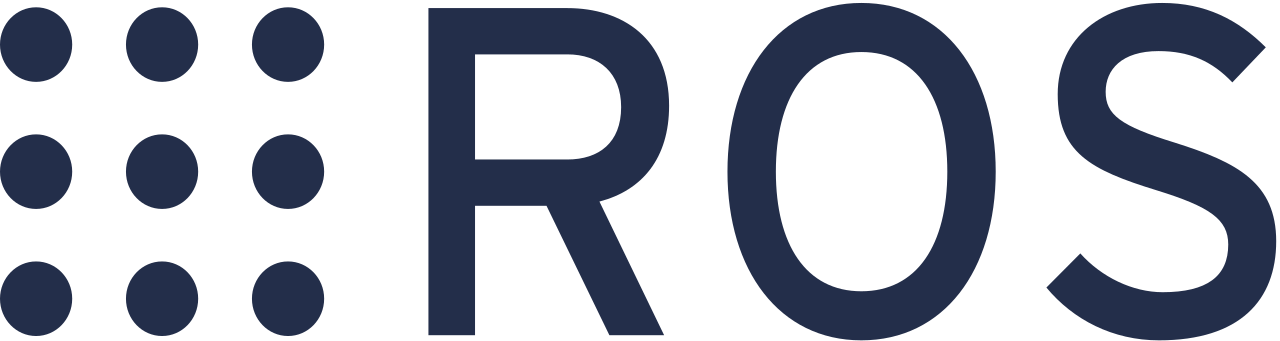
\includegraphics[valign=c,width=\textwidth]{./figure/ROS.png}
	\end{minipage}
	\begin{minipage}[t]{0.5\textwidth}
		
\includegraphics[valign=c,width=\textwidth]{./figure/GAZEBO.png}
	\end{minipage}
\end{figure}